\section*{Методы отбора признаков. Качество классификации.}
Рассмотрим задачу бинарной классификации с обучающей выборкой $D = \{(x_i, y_i)\}_{i=1}^n$, где $x_i \in \mathbb{R}^d$ --- вектор признаков, $y_i \in \{0, 1\}$ --- бинарная переменная.
Мы хотим построить модель $f: \mathbb{R}^d \to \{0, 1\}$, которая принимает на вход вектор признаков и выдает предсказание класса.
Есть следующие способы измерять качество модели:

Accuracy

Precision

Recall

$F_{\beta}$ score

ROC AUC

Для каждого объекта из выборки мы имеем 4 варианта разивития событий:

TP --- True Positive, классификатор предсказал 1, верное значение тоже 1

FP --- False Positive, классификатор предсказал 1, верное значение 0

TN --- True Negative, классификатор предсказал 0, верное значение тоже 0

FN --- False Negative, классификатор предсказал 0, верное значение 1


Ясно, что мы хотим видеть как можно больше TP и TN и как можно меньше FP и FN.

Accuracy --- это доля правильных ответов классификатора.
$$
    \text{Accuracy} = \frac{TP + TN}{TP + FP + TN + FN} = \frac{1}{n} \sum_{i=1}^n \mathbb{I}(y_i = f(x_i))
$$

Достаточно банальная метрика, которая не учитывает дисбаланса классов, но в качестве базового варианта подходит отлично.

Precision --- это доля объектов, которые классификатор предсказал как 1, среди всех объектов, которые он предсказал как 1.
$$
    \text{Precision} = \frac{TP}{TP + FP}
$$

Recall --- это доля объектов, которые классификатор предсказал как 1, среди всех объектов, которые действительно равны 1.
$$
    \text{Recall} = \frac{TP}{TP + FN}
$$

Precision и Recall --- базовые метрики, но по отдельности их использовать нельзя, поэтому придумали $F_{\beta}$ score.

$F_{\beta}$ score --- это взвешенное среднее гармоническое precision и recall.
$$
    F_{\beta} = (1 + \beta^2) \frac{precision \cdot recall}{\beta^2 \cdot precision + recall}
$$

$TPR$ --- это доля объектов, которые классификатор предсказал как 1, среди всех объектов, которые действительно равны 1.
$$
    TPR = \frac{TP}{TP + FN}
$$

$FPR$ --- это доля объектов, которые классификатор предсказал как 1, среди всех объектов, которые действительно равны 0.
$$
    FPR = \frac{FP}{FP + TN}
$$

Обычно, когда мы решаем задачу бинарной классификации, то мы не предсказываем явный класс, а предсказываем какое-то значение, и чем больше это значение, тем больше вероятность того, что объект принадлежит к классу 1.
Следовательно, мы можем устанавливать пороговое значение, которое будет определять, к какому классу отнести объект.
При увеличении порога отсечения мы увеличиваем количество объектов, которые отнесены к классу 0, и уменьшаем количество объектов, которые отнесены к классу 1.
Заметим, что также при увеличении порога отсечения TPR и FPR будут уменьшаться.

ROC кривая --- это кривая, которая показывает зависимость TPR от FPR при изменении порога отсечения. То есть по оси $x$ откладывается $FPR$, а по оси $y$ --- $TPR$.

Строго говоря, ROC кривая --- это множество точек вида $(FPR(t), TPR(t))$, где $t$ --- пороговое значение вероятности.

ROC-AUC --- это площадь под ROC кривой.

\subsection*{Задача 1}

Мы хотим построить модель бинарной классификации, которая будет по некоторому описанию пациента предсказывать, болен ли он раком.
В случае, если наша модель скажет, что пациент болен раком, то мы отправим его на дополнительное обследование, что обойдется пациенту в некоторую неприятную, но не критичную сумму денег.
Если же наша модель скажет, что пациент здоров, то мы ничего не будем предпринимать.
Мы хотим выбрать метрику качества для нашей модели из следующего списка: Accuracy, Precision, Recall, $F_{\beta}$ score, что нам лучше всего подойдет?
Если мы хотим выбрать $F_{\beta}$ score, то какие значения $\beta$ нам лучше всего подойдут?

\begin{solution}
Accuracy --- не лучший вариант, так как ошибка FP и FN в нашем случае не равнозначны.
Не отправить больного на дополнительное обследование значительно хуже, чем отправить здорового пациента на обследование.
Precision и Recall --- достаточно плохие метрики, ведь есть очень простая модель, которая даст 100\% Precision --- просто предсказывать, что все пациенты больны, аналогичная проблема и с Recall.
$F_{\beta}$ score --- отличный вариант, ведь с помощью $\beta$ мы можем выбирать, какое предпочтение мы отдаем Precision, а какое Recall.
В нашем случае, мы хотим, чтобы Precision был предпочтительнее Recall, поэтому $\beta$ должно быть меньше 1.
Если мы для себя решили, что смерть человека стоит как 10 дообследований, то стоит брать $\beta = \frac{1}{10}$.
\end{solution}
\subsection*{Задача 2}
Предположим, что мы измеряем качество модели с помощью ROC-AUC. Допустим, что у нас есть две модели, чьи ROC кривые выглядят следующим образом:
\begin{figure}[h]
    \centering
    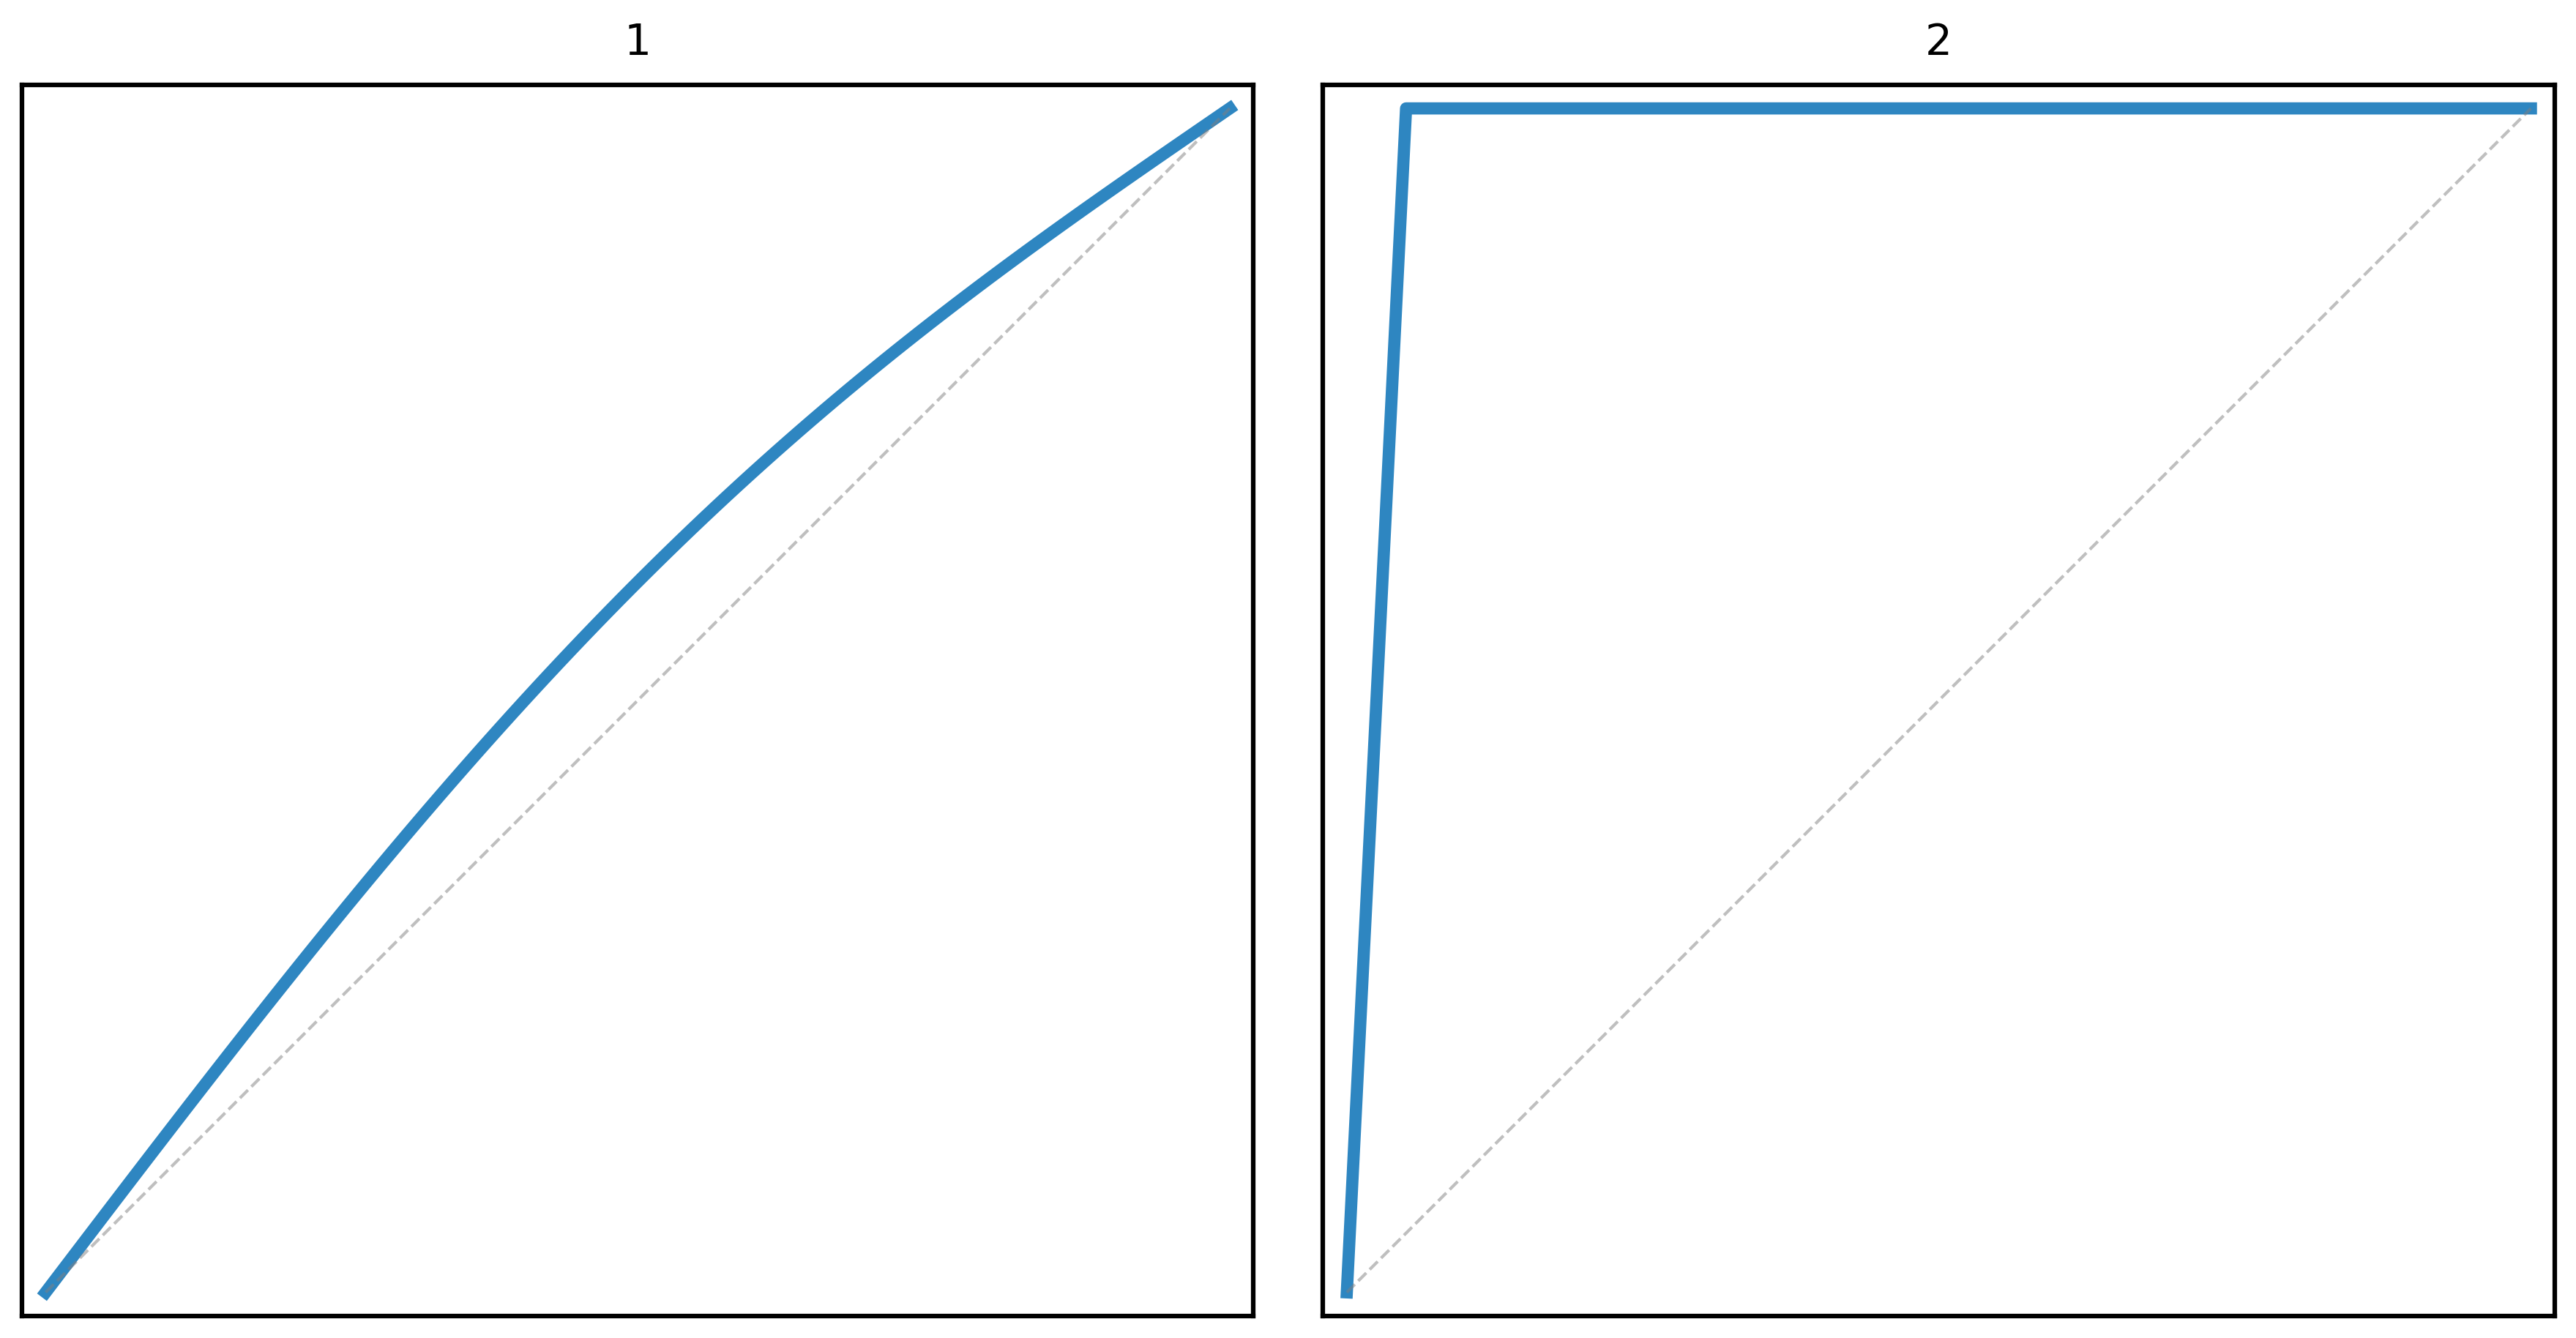
\includegraphics[width=0.8\textwidth]{roc_curves_comparison_1.png}
    \caption{Две ROC кривые}
\end{figure}
Как эти модели упорядочить по качеству?

\begin{solution}
Первая модель самая худшая, ведь ее ROC кривая максимально близка к диагонали, значит она имеет миниимальную ROC-AUC.
Это плохо, но что по смыслу означает близкая к диагонали ROC кривая?

Это означает, что для любого порога отсечения $t$ имеем примерно $TPR(t) = FPR(t)$.
Что означает $TPR(t) = FPR(t)$? Это означает, что модель просто случайным образом с вероятностью $TPR(t)=FPR(t)$ предсказывает 1 класс.
Вторая модель лучшая, но почему?

А что означает график, который близок к уголку, как на рисунке 2?
Это означает, что мы можем взять такой порог отсечения $t$, что почти выполнено $TPR(t) = 1$ и $FPR(t) = 0$.
А это идеальная модель, которая никогда не ошибается.

Заметим, что чем больше площадь под ROC кривой, тем ближе эта кривая к уголку, а значит тем лучше модель.
\end{solution}
\subsection*{Задача 3}
Продолжим измерять качество моделей с помощью ROC-AUC. Допустим, что у нас есть две модели, чьи ROC кривые выглядят следующим образом:
\begin{figure}[h]
    \centering
    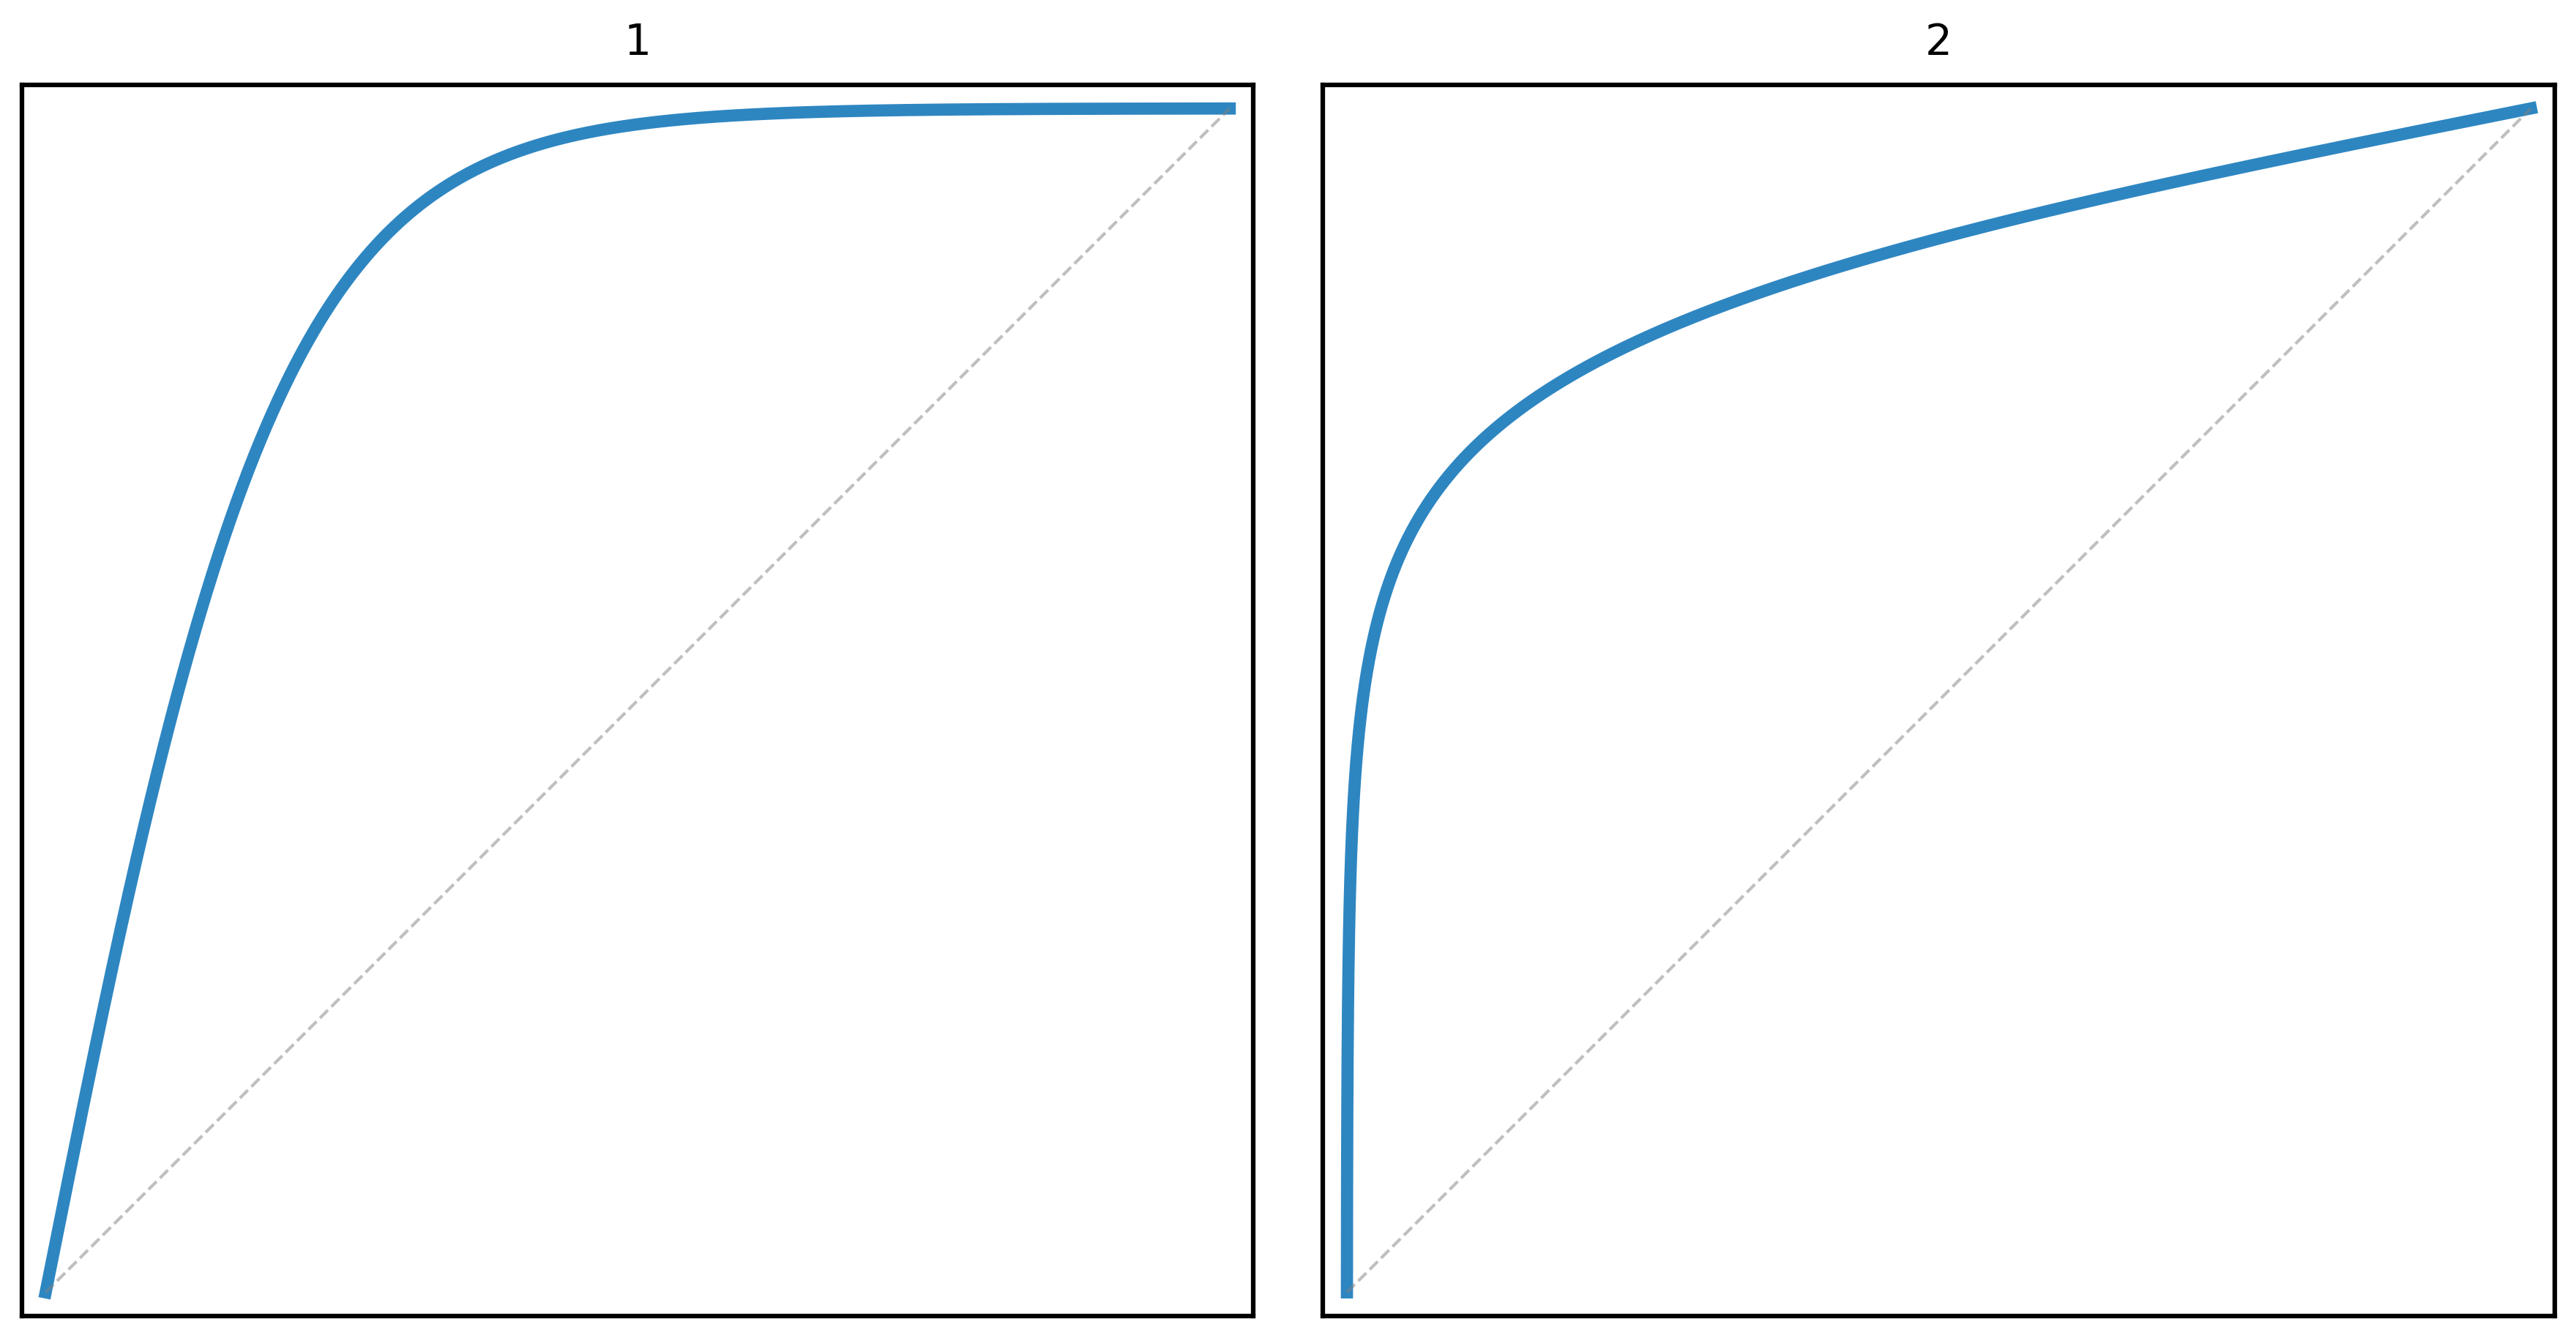
\includegraphics[width=0.8\textwidth]{roc_curves_comparison_2.png}
    \caption{Две ROC кривые}
\end{figure}
Как эти модели упорядочить по качеству? А как выбрать порог отсечения? В чем преимущество ROC перед $F_{\beta}$ score?

\begin{solution}
В данном случае, обе ROC кривые имеют одинаковую площадь под графиком, а значит одинаковую ROC-AUC, поэтому просто посмотреть на метрику ROC-AUC нельзя.
На самом деле, однозначного ответа нет, всё зависит от конкретной задачи.

Первая кривая быстро достигает высокого значения TPR, при не самом высоком значении FPR.

Это означает, что выбрав порог отсечения $t$, при котором $TPR(t)$ будет близок к 1, а $FPR(t)$ будет близок к 0.5, мы получим модель,
которая угадывает почти всех, кто попадает в 1 класс, но при этом не сильно много ошибается на классе 0.
Такая модель отлично подойдет в первой задаче, где мы хотим отгадать почти всех больных, но при этом не сильно много отправлять на дополнительное обследование здоровых людей.

На втором графике ситуация обратная, мы можем выбрать порог отсечения $t$, при котором $TPR(t)$ будет близок к 0.5, а $FPR(t)$ будет близок к 1.
Такая модель будет полезна в случае, когда мы хотим минимизировать количество ошибок на классе 0, но при этом не сильно много ошибаться на классе 1.
В контексте первой задачи, это означает, что мы не хотим тратить лишние деньги на дополнительное обследование здоровых людей даже ценой смерти больных, которых мы не отправляем на дополнительное обследование.

Исходя из этих примеров, становится понятно, как стоит выбирать порог отсечения. По сути его выбор означает, насколько мы готовы пожертвовать ошибками на предсказаниях одного класса, чтобы минимизировать ошибки на предсказаниях другого класса.
Это такой аналог $\beta$ в $F_{\beta}$ score, только $\beta$ мы выбирали до измерения метрики, а в случае ROC кривой мы выбираем порог отсечения глядя на график и имея какую-то дополнительную информацию о том, как работает модель при разных порогах.
Это может быть очень полезно, ведь далеко не всегда мы готовы определиться с балансом ошибок на классах перед тем, как начать решать задачу.
\end{solution}
